\documentclass[Ex4_Zusammenfassung.tex]{subfiles}

\begin{document}

\section{Angeregte Zustände in Atomkernen}
\textbf{von \hein \& \martina}\\

\subsection*{Rückblick}
Bei 2--atomigen Molekülen sind verschiedene Formen der Anregung möglich. Die niedrigsten angeregten Zustände sind Rotationen, außerdem sind auch Vibrationen möglich. Vibrationsanregungen haben deutlich höhere Energien als Rotationsanregungen: $E_{\text{Vib}}  \simeq 100\cdot E_{\text{Rot}}$

\subsection{Angeregte Zustände}
Kerne mit abgeschlossenen Schalen sind kugelsymmetrisch. In der Nähe abgeschlossener Schalen wird ein Kern immer noch am besten durch das Schalenmodell beschrieben. Ist die Schale nicht abgeschlossen, ist der Kern nicht mehr kugelsymmetrisch, sondern ähnelt einem Ellipsoid. 
\begin{figure}[h]
	\begin{subfigure}[t]{0.3\textwidth}
		\centering
		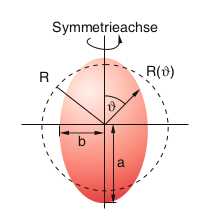
\includegraphics[scale=0.55, trim= 0 -0.45cm 0 0]{ellipsoid_1.png}
	\end{subfigure}
	~
	\begin{subfigure}[b]{0.7\textwidth}
		\centering
		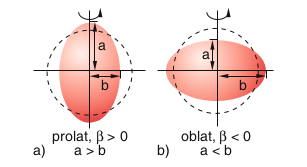
\includegraphics[scale=0.6]{ellipsoid_2.png}
	\end{subfigure}
	\caption{Allgemeine Beschreibung der Ellipsoiden (links), und die Bezeichnungen für die 2 verschiedenen Formen (rechts, a und b)}
	\label{ellipsoids}
\end{figure}
Ein rotationssymmetrischer Ellipsoid kann durch Polardarstellung dargestellt werden:
\begin{align}
	R(\vartheta) &= R_0 \left[ 1 + \beta \cdot Y_2^0 (\cos \vartheta ) \right], \quad \beta \ll 1\\
	R_k &= R_0 \cdot \left[ 1 + \sqrt{\frac{5}{4\pi}} \beta \cos\lp \vartheta - \frac{2 \pi k}{3}\rp  \right]
\end{align}
wobei $\beta$ einen Deformationsparameter darstellt. 

Dabei treten zwei Formen auf: Oblaten und Prolaten (Abb. \ref{ellipsoids} rechts). 

\subsection{Rotation}
Da in den Kernspektren äquidistante Linien auftauchen, schließt man nun auf Rotationsanregungen. Durch Stöße mit schweren Projektilen (Protonen, $\alpha$--Teilchen) können Drehimpulse erzeugt und der Kern damit zu Rotation angeregt werden. Da auf kugelsymmetrische Objekte kein Drehimpuls übertragen werden kann, werden die Kerne als deformiert angenommen. 
\begin{figure}[h]
	\centering
	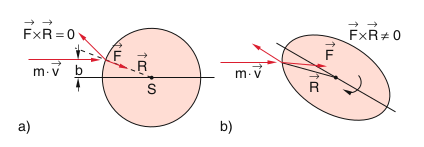
\includegraphics[scale=0.4]{deformiert.png}
	\caption{Kein Drehimpulsübertrag bei kugelsymmetrischem Kern (a), Drehimpulsübertrag auf deformierten Kern (b).}
\end{figure}
Entsprechend steht die Rotationsachse immer senkrecht auf der Symmetrieachse, da sonst wie bei der Kugel kein Drehmoment wirken kann. 

Die Energieniveaus eines quantenmechanischen Rotators sind
\begin{equation}
	E = \frac{\hslash^2}{2 \Theta} I (I+1)
\end{equation}
wobei $\Theta$ das Trägheitsmoment und $I$ die Drehimpulsquantenzahl des Kerns darstellen. 

Aus den Abständen zwischen zwei Spektrallinien lässt sich $\Theta$ ermitteln. Aufgrund der Paritätserhaltung sind nur gerade Werte für $I$ erlaubt:
\begin{align}
	\intertext{hierfür sei} A = \frac{\hslash^2}{2 \Theta}
	\intertext{und somit folgt}
	\Delta E = E_I - E_{I-2} &= AI(I+1) - A(I-2)(I-1)\\
	&= A(I^2 + I - I^2 + 3I - 2)\\
	&= A(4I - 2)\\
	&= 4AI - 2A
\end{align}
$\Delta E$ entspricht einer Spektrallinie. Also folgt für die Differenz zweier Spektrallinien:
\begin{align}
	\Delta (\Delta E) &= 4A(I+2) -2A - 4AI + 2A\\
	&= 4AI + 8A - 4AI \\
	&= 8A = 8 \frac{\hslash^2}{2\Theta}
\end{align}
Die berechneten $\Theta$ sind um den Faktor 2 zu groß, da man den Kern nicht als starren Rotator annehmen kann. 
\subsection{Vibration}
kann auch bei kugelsymmetrischen Kernen auftreten. Dabei gibt es 2 wesentliche Schwingungstypen:
\begin{itemize}
	\item Radiale Kompressionssschwingung:\\
	Die Dichte des Kerns ändert sich periodisch und es tritt kein Drehimpuls auf. Da die Kernmaterie aber fast inkompressibel ist, muss die Anregungsenergie hierfür sehr groß sein.
	\item Oberflächenschwingung:\\
	Das Kernvolumen ändert sich nicht, aber der Kern wird deformiert. Hier kann z.B. die Kugel abwechselnd in Oblate und Prolate übergehen.
\end{itemize}
Abhängig von der Art der Schwingung erhält man bei genügend kleinen Amplituden die Energiewerte des harmonischen Oszillators:
\begin{equation}
	E_{\text{Vib}} = \hslash \omega_{\ell, m} \lp n + \frac{1}{2} \rp
\end{equation}
$\omega_{\ell, m}$ hängt von der Art der Schwingung und Deformation ab.
\end{document}